% Options for packages loaded elsewhere
\PassOptionsToPackage{unicode}{hyperref}
\PassOptionsToPackage{hyphens}{url}
%
\documentclass[
]{article}
\usepackage{lmodern}
\usepackage{amssymb,amsmath}
\usepackage{ifxetex,ifluatex}
\ifnum 0\ifxetex 1\fi\ifluatex 1\fi=0 % if pdftex
  \usepackage[T1]{fontenc}
  \usepackage[utf8]{inputenc}
  \usepackage{textcomp} % provide euro and other symbols
\else % if luatex or xetex
  \usepackage{unicode-math}
  \defaultfontfeatures{Scale=MatchLowercase}
  \defaultfontfeatures[\rmfamily]{Ligatures=TeX,Scale=1}
\fi
% Use upquote if available, for straight quotes in verbatim environments
\IfFileExists{upquote.sty}{\usepackage{upquote}}{}
\IfFileExists{microtype.sty}{% use microtype if available
  \usepackage[]{microtype}
  \UseMicrotypeSet[protrusion]{basicmath} % disable protrusion for tt fonts
}{}
\makeatletter
\@ifundefined{KOMAClassName}{% if non-KOMA class
  \IfFileExists{parskip.sty}{%
    \usepackage{parskip}
  }{% else
    \setlength{\parindent}{0pt}
    \setlength{\parskip}{6pt plus 2pt minus 1pt}}
}{% if KOMA class
  \KOMAoptions{parskip=half}}
\makeatother
\usepackage{xcolor}
\IfFileExists{xurl.sty}{\usepackage{xurl}}{} % add URL line breaks if available
\IfFileExists{bookmark.sty}{\usepackage{bookmark}}{\usepackage{hyperref}}
\hypersetup{
  pdftitle={rintrinio},
  pdfauthor={Team Andrey Markov},
  hidelinks,
  pdfcreator={LaTeX via pandoc}}
\urlstyle{same} % disable monospaced font for URLs
\usepackage[margin=1in]{geometry}
\usepackage{color}
\usepackage{fancyvrb}
\newcommand{\VerbBar}{|}
\newcommand{\VERB}{\Verb[commandchars=\\\{\}]}
\DefineVerbatimEnvironment{Highlighting}{Verbatim}{commandchars=\\\{\}}
% Add ',fontsize=\small' for more characters per line
\usepackage{framed}
\definecolor{shadecolor}{RGB}{248,248,248}
\newenvironment{Shaded}{\begin{snugshade}}{\end{snugshade}}
\newcommand{\AlertTok}[1]{\textcolor[rgb]{0.94,0.16,0.16}{#1}}
\newcommand{\AnnotationTok}[1]{\textcolor[rgb]{0.56,0.35,0.01}{\textbf{\textit{#1}}}}
\newcommand{\AttributeTok}[1]{\textcolor[rgb]{0.77,0.63,0.00}{#1}}
\newcommand{\BaseNTok}[1]{\textcolor[rgb]{0.00,0.00,0.81}{#1}}
\newcommand{\BuiltInTok}[1]{#1}
\newcommand{\CharTok}[1]{\textcolor[rgb]{0.31,0.60,0.02}{#1}}
\newcommand{\CommentTok}[1]{\textcolor[rgb]{0.56,0.35,0.01}{\textit{#1}}}
\newcommand{\CommentVarTok}[1]{\textcolor[rgb]{0.56,0.35,0.01}{\textbf{\textit{#1}}}}
\newcommand{\ConstantTok}[1]{\textcolor[rgb]{0.00,0.00,0.00}{#1}}
\newcommand{\ControlFlowTok}[1]{\textcolor[rgb]{0.13,0.29,0.53}{\textbf{#1}}}
\newcommand{\DataTypeTok}[1]{\textcolor[rgb]{0.13,0.29,0.53}{#1}}
\newcommand{\DecValTok}[1]{\textcolor[rgb]{0.00,0.00,0.81}{#1}}
\newcommand{\DocumentationTok}[1]{\textcolor[rgb]{0.56,0.35,0.01}{\textbf{\textit{#1}}}}
\newcommand{\ErrorTok}[1]{\textcolor[rgb]{0.64,0.00,0.00}{\textbf{#1}}}
\newcommand{\ExtensionTok}[1]{#1}
\newcommand{\FloatTok}[1]{\textcolor[rgb]{0.00,0.00,0.81}{#1}}
\newcommand{\FunctionTok}[1]{\textcolor[rgb]{0.00,0.00,0.00}{#1}}
\newcommand{\ImportTok}[1]{#1}
\newcommand{\InformationTok}[1]{\textcolor[rgb]{0.56,0.35,0.01}{\textbf{\textit{#1}}}}
\newcommand{\KeywordTok}[1]{\textcolor[rgb]{0.13,0.29,0.53}{\textbf{#1}}}
\newcommand{\NormalTok}[1]{#1}
\newcommand{\OperatorTok}[1]{\textcolor[rgb]{0.81,0.36,0.00}{\textbf{#1}}}
\newcommand{\OtherTok}[1]{\textcolor[rgb]{0.56,0.35,0.01}{#1}}
\newcommand{\PreprocessorTok}[1]{\textcolor[rgb]{0.56,0.35,0.01}{\textit{#1}}}
\newcommand{\RegionMarkerTok}[1]{#1}
\newcommand{\SpecialCharTok}[1]{\textcolor[rgb]{0.00,0.00,0.00}{#1}}
\newcommand{\SpecialStringTok}[1]{\textcolor[rgb]{0.31,0.60,0.02}{#1}}
\newcommand{\StringTok}[1]{\textcolor[rgb]{0.31,0.60,0.02}{#1}}
\newcommand{\VariableTok}[1]{\textcolor[rgb]{0.00,0.00,0.00}{#1}}
\newcommand{\VerbatimStringTok}[1]{\textcolor[rgb]{0.31,0.60,0.02}{#1}}
\newcommand{\WarningTok}[1]{\textcolor[rgb]{0.56,0.35,0.01}{\textbf{\textit{#1}}}}
\usepackage{graphicx}
\makeatletter
\def\maxwidth{\ifdim\Gin@nat@width>\linewidth\linewidth\else\Gin@nat@width\fi}
\def\maxheight{\ifdim\Gin@nat@height>\textheight\textheight\else\Gin@nat@height\fi}
\makeatother
% Scale images if necessary, so that they will not overflow the page
% margins by default, and it is still possible to overwrite the defaults
% using explicit options in \includegraphics[width, height, ...]{}
\setkeys{Gin}{width=\maxwidth,height=\maxheight,keepaspectratio}
% Set default figure placement to htbp
\makeatletter
\def\fps@figure{htbp}
\makeatother
\setlength{\emergencystretch}{3em} % prevent overfull lines
\providecommand{\tightlist}{%
  \setlength{\itemsep}{0pt}\setlength{\parskip}{0pt}}
\setcounter{secnumdepth}{-\maxdimen} % remove section numbering
\newlength{\cslhangindent}
\setlength{\cslhangindent}{1.5em}
\newenvironment{cslreferences}%
  {\setlength{\parindent}{0pt}%
  \everypar{\setlength{\hangindent}{\cslhangindent}}\ignorespaces}%
  {\par}

\title{rintrinio}
\author{Team Andrey Markov}
\date{}

\begin{document}
\maketitle

\hypertarget{introduction-to-rintrinio}{%
\section{Introduction to rintrinio}\label{introduction-to-rintrinio}}

The purpose of rintrinio is to take the data from Intrinio (Swagger
Codegen community 2020) and make it extraordinarily easy to move to a
format for analysis in R (R Core Team 2019).

This document introduces you to the functions included in this package.

\hypertarget{functions}{%
\subsection{Functions}\label{functions}}

The four functions in the package are as follows:

\begin{itemize}
\tightlist
\item
  \texttt{gather\_financial\_statement\_time\_series()} to compare a
  single company's financial statements over time
\item
  \texttt{gather\_financial\_statement\_company\_compare()} to compare
  multiple company's financial statements in a single period
\item
  \texttt{gather\_stock\_time\_series()} to gather a time series of
  stock price information
\item
  \texttt{gather\_stock\_returns()} to gather returns of stocks over
  time
\end{itemize}

\hypertarget{time-series-financial-statement-analysis-with-gather_financial_statement_time_series}{%
\subsubsection{\texorpdfstring{Time Series Financial Statement Analysis
with
\texttt{gather\_financial\_statement\_time\_series()}}{Time Series Financial Statement Analysis with gather\_financial\_statement\_time\_series()}}\label{time-series-financial-statement-analysis-with-gather_financial_statement_time_series}}

\texttt{gather\_financial\_statement\_time\_series()} takes in
information that would be spread across multiple lines when querying the
Intrinio API directly, and puts it into a function that by default
returns a dataframe that is ready to be used for analysis. This function
should be used for time series analysis of financial statements (income
statement, balance sheet, or cash flow statement).

For example, we can compare Apple's 2018 and 2019 Q1 Balance Sheet:

\begin{Shaded}
\begin{Highlighting}[]
\NormalTok{fs\_ts \textless{}{-}}\StringTok{ }\KeywordTok{gather\_financial\_statement\_time\_series}\NormalTok{(}\DataTypeTok{api\_key =}\NormalTok{ api\_key, }
                                                \DataTypeTok{ticker =} \StringTok{\textquotesingle{}AAPL\textquotesingle{}}\NormalTok{,}
                                                \DataTypeTok{statement =} \StringTok{\textquotesingle{}balance\_sheet\_statement\textquotesingle{}}\NormalTok{, }
                                                \DataTypeTok{year =} \KeywordTok{c}\NormalTok{(}\StringTok{"2018"}\NormalTok{, }\StringTok{"2019"}\NormalTok{), }
                                                \DataTypeTok{period =} \KeywordTok{c}\NormalTok{(}\StringTok{\textquotesingle{}Q1\textquotesingle{}}\NormalTok{))}

\NormalTok{knitr}\OperatorTok{::}\KeywordTok{kable}\NormalTok{(fs\_ts)}
\end{Highlighting}
\end{Shaded}

\begin{tabular}{l|l|l}
\hline
type & fin\_value & fin\_value.\\
\hline
ticker & AAPL & AAPL\\
\hline
statement & balance\_sheet\_statement & balance\_sheet\_statement\\
\hline
year & 2018 & 2019\\
\hline
period & Q1 & Q1\\
\hline
cashandequivalents & 2.7491e+10 & 4.4771e+10\\
\hline
shortterminvestments & 4.9662e+10 & 4.1656e+10\\
\hline
notereceivable & 2.7459e+10 & 1.8904e+10\\
\hline
accountsreceivable & 2.344e+10 & 1.8077e+10\\
\hline
netinventory & 4.421e+09 & 4.988e+09\\
\hline
othercurrentassets & 1.1337e+10 & 1.2432e+10\\
\hline
totalcurrentassets & 1.4381e+11 & 1.40828e+11\\
\hline
netppe & 3.3679e+10 & 3.9597e+10\\
\hline
longterminvestments & 2.07944e+11 & 1.58608e+11\\
\hline
goodwill & 5.889e+09 & NA\\
\hline
intangibleassets & 2.149e+09 & NA\\
\hline
othernoncurrentassets & 1.3323e+10 & 3.4686e+10\\
\hline
totalnoncurrentassets & 2.29305e+11 & 1.93294e+11\\
\hline
totalassets & 4.06794e+11 & 3.73719e+11\\
\hline
shorttermdebt & -1.8478e+10 & -2.1741e+10\\
\hline
accountspayable & -6.2985e+10 & -4.4293e+10\\
\hline
accruedexpenses & -2.6281e+10 & NA\\
\hline
currentdeferredrevenue & -8.044e+09 & -5.546e+09\\
\hline
totalcurrentliabilities & -1.15788e+11 & -1.08283e+11\\
\hline
longtermdebt & -1.03922e+11 & -9.2989e+10\\
\hline
noncurrentdeferredrevenue & -3.131e+09 & NA\\
\hline
othernoncurrentliabilities & -4.3754e+10 & -5.4555e+10\\
\hline
totalnoncurrentliabilities & -1.50807e+11 & -1.47544e+11\\
\hline
totalliabilities & -2.66595e+11 & -2.55827e+11\\
\hline
commitmentsandcontingencies & 0 & 0\\
\hline
commonequity & -3.6447e+10 & -4.097e+10\\
\hline
retainedearnings & -1.04593e+11 & -8.051e+10\\
\hline
aoci & 8.41e+08 & 3.588e+09\\
\hline
totalcommonequity & -1.40199e+11 & -1.17892e+11\\
\hline
totalequity & -1.40199e+11 & -1.17892e+11\\
\hline
totalequityandnoncontrollinginterests & -1.40199e+11 & -1.17892e+11\\
\hline
totalliabilitiesandequity & -4.06794e+11 & -3.73719e+11\\
\hline
othercurrentliabilities & NA & -3.6703e+10\\
\hline
\end{tabular}

\hypertarget{cross-company-financial-statement-analysis-with-gather_financial_statement_company_compare}{%
\subsubsection{\texorpdfstring{Cross-Company Financial Statement
Analysis with
\texttt{gather\_financial\_statement\_company\_compare()}}{Cross-Company Financial Statement Analysis with gather\_financial\_statement\_company\_compare()}}\label{cross-company-financial-statement-analysis-with-gather_financial_statement_company_compare}}

\texttt{gather\_financial\_statement\_company\_compare()} takes in
information that would be spread across multiple lines when querying the
Intrinio API directly, and puts it into a function that by default
returns a dataframe that is ready to be used for analysis. This function
should be used for cross-company analysis of financial statements
(income statement, balance sheet, or cash flow statement).

For example, we can compare Apple and Cisco's Income Statement results
for Q1 of 2019:

\begin{Shaded}
\begin{Highlighting}[]
\NormalTok{fs\_compare \textless{}{-}}\StringTok{ }\KeywordTok{gather\_financial\_statement\_company\_compare}\NormalTok{(}\DataTypeTok{api\_key =}\NormalTok{ api\_key, }
                                                         \DataTypeTok{ticker =} \KeywordTok{c}\NormalTok{(}\StringTok{"AAPL"}\NormalTok{, }\StringTok{"CSCO"}\NormalTok{), }
                                                         \DataTypeTok{statement =} \StringTok{"income\_statement"}\NormalTok{, }
                                                         \DataTypeTok{year =} \StringTok{"2019"}\NormalTok{, }
                                                         \DataTypeTok{period =} \StringTok{"Q1"}\NormalTok{)}

\NormalTok{knitr}\OperatorTok{::}\KeywordTok{kable}\NormalTok{(fs\_compare)}
\end{Highlighting}
\end{Shaded}

\begin{tabular}{l|l|l}
\hline
name & value.x & value.y\\
\hline
ticker & AAPL & CSCO\\
\hline
statement & income\_statement & income\_statement\\
\hline
year & 2019 & 2019\\
\hline
period & Q1 & Q1\\
\hline
operatingrevenue & -8.431e+10 & -1.3072e+10\\
\hline
totalrevenue & -8.431e+10 & -1.3072e+10\\
\hline
operatingcostofrevenue & 5.2279e+10 & 4.926e+09\\
\hline
totalcostofrevenue & 5.2279e+10 & 4.926e+09\\
\hline
totalgrossprofit & -3.2031e+10 & -8.146e+09\\
\hline
sgaexpense & 4.783e+09 & 2.11e+08\\
\hline
rdexpense & 3.902e+09 & 1.608e+09\\
\hline
totaloperatingexpenses & 8.685e+09 & 4.341e+09\\
\hline
totaloperatingincome & -2.3346e+10 & -3.805e+09\\
\hline
otherincome & -5.6e+08 & 1.9e+07\\
\hline
totalotherincome & -5.6e+08 & -1.04e+08\\
\hline
totalpretaxincome & -2.3906e+10 & -3.909e+09\\
\hline
incometaxexpense & 3.941e+09 & 3.6e+08\\
\hline
netincomecontinuing & -1.9965e+10 & -3.549e+09\\
\hline
netincome & -1.9965e+10 & -3.549e+09\\
\hline
netincometocommon & -1.9965e+10 & -3.549e+09\\
\hline
weightedavebasicsharesos & -4735820000 & -4.565e+09\\
\hline
basiceps & -4.22 & -0.78\\
\hline
weightedavedilutedsharesos & -4773252000 & -4.614e+09\\
\hline
dilutedeps & -4.18 & -0.77\\
\hline
weightedavebasicdilutedsharesos & -4.731e+09 & -4.55e+09\\
\hline
basicdilutedeps & -4.22 & -0.78\\
\hline
cashdividendspershare & -0.73 & -0.33\\
\hline
marketingexpense & NA & 2.41e+09\\
\hline
amortizationexpense & NA & 3.4e+07\\
\hline
restructuringcharge & NA & 7.8e+07\\
\hline
totalinterestexpense & NA & 2.21e+08\\
\hline
totalinterestincome & NA & -3.44e+08\\
\hline
\end{tabular}

\hypertarget{time-series-stock-analysis-with-gather_stock_time_series}{%
\subsubsection{\texorpdfstring{Time Series Stock Analysis with
\texttt{gather\_stock\_time\_series()}}{Time Series Stock Analysis with gather\_stock\_time\_series()}}\label{time-series-stock-analysis-with-gather_stock_time_series}}

\texttt{gather\_stock\_time\_series()} is a function for simplifying
time series analysis of stock prices of a single company. It takes in
the ticker, start and end dates (optional), and an Intrinio API key, and
returns a dataframe that can easily be plotted to view trend analysis,
or analysed as is.

For example, we can see how Cisco's close price changed over 2019 and
model it with ggplot (Wickham 2016):

\begin{Shaded}
\begin{Highlighting}[]
\NormalTok{stock\_data \textless{}{-}}\StringTok{ }\KeywordTok{gather\_stock\_time\_series}\NormalTok{(}\DataTypeTok{api\_key =}\NormalTok{ api\_key, }
                                       \DataTypeTok{ticker =} \StringTok{"CSCO"}\NormalTok{, }
                                       \DataTypeTok{start\_date =} \StringTok{"2019{-}01{-}01"}\NormalTok{, }
                                       \DataTypeTok{end\_date =} \StringTok{"2019{-}12{-}31"}\NormalTok{,}
                                       \DataTypeTok{allow\_max\_rows =} \OtherTok{TRUE}\NormalTok{)}

\KeywordTok{ggplot}\NormalTok{(stock\_data, }\KeywordTok{aes}\NormalTok{(}\DataTypeTok{x =}\NormalTok{ date, }\DataTypeTok{y =}\NormalTok{ close)) }\OperatorTok{+}
\StringTok{  }\KeywordTok{geom\_line}\NormalTok{() }\OperatorTok{+}
\StringTok{  }\KeywordTok{ggtitle}\NormalTok{(}\StringTok{"Cisco Close Prices over 2019"}\NormalTok{) }\OperatorTok{+}
\StringTok{  }\KeywordTok{labs}\NormalTok{(}\DataTypeTok{x =} \StringTok{"Time"}\NormalTok{, }\DataTypeTok{y =} \StringTok{"Close Price"}\NormalTok{)}
\end{Highlighting}
\end{Shaded}

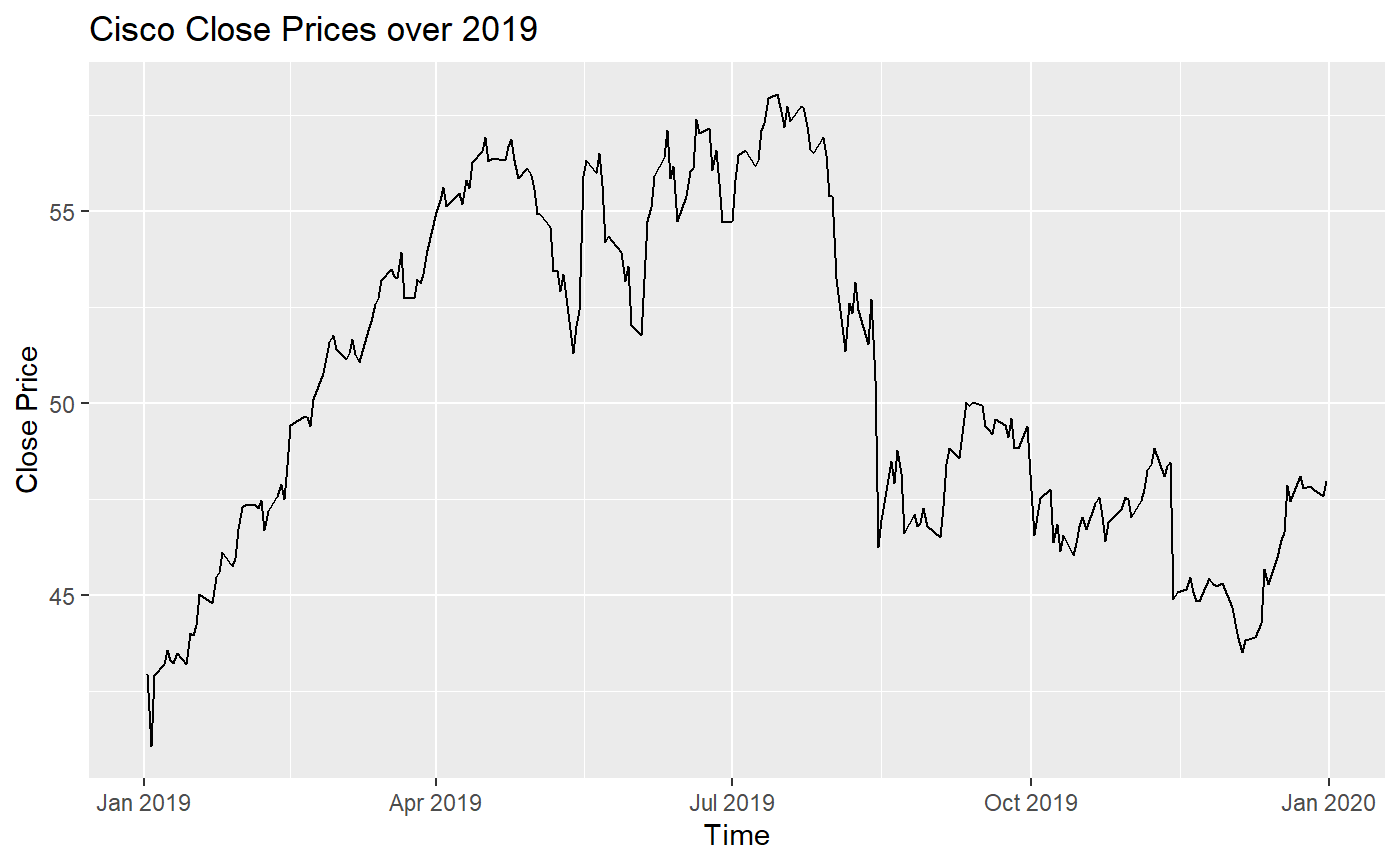
\includegraphics{rintrinio-vignette_files/figure-latex/gather_stock_time_series-1.pdf}

\hypertarget{understand-stock-returns-with-gather_stock_returns}{%
\subsubsection{\texorpdfstring{Understand Stock Returns with
\texttt{gather\_stock\_returns()}}{Understand Stock Returns with gather\_stock\_returns()}}\label{understand-stock-returns-with-gather_stock_returns}}

\texttt{gather\_stock\_returns()} allows for a combination of looking at
time series stock data and comparing returns across companies. This
function allows effortless comparisons of returns across companies given
a buy date and a sell date. Historical analysis is important for
portfolio evaluations and comparisons.

For example, we can compare Apple and Cisco's returns over Q1 2019:

\begin{Shaded}
\begin{Highlighting}[]
\NormalTok{stock\_returns \textless{}{-}}\StringTok{ }\KeywordTok{gather\_stock\_returns}\NormalTok{(}\DataTypeTok{api\_key =}\NormalTok{ api\_key, }
                                      \DataTypeTok{ticker =} \KeywordTok{c}\NormalTok{(}\StringTok{"AAPL"}\NormalTok{, }\StringTok{"CSCO"}\NormalTok{), }
                                      \DataTypeTok{buy\_date =} \StringTok{"2019{-}01{-}01"}\NormalTok{, }
                                      \DataTypeTok{sell\_date =} \StringTok{"2019{-}03{-}31"}\NormalTok{)}

\NormalTok{knitr}\OperatorTok{::}\KeywordTok{kable}\NormalTok{(stock\_returns)}
\end{Highlighting}
\end{Shaded}

\begin{tabular}{l|l|r|l|r|r}
\hline
Stock & Buy.date & Buy.price & Sell.date & Sell.price & Return....\\
\hline
AAPL & 2019-01-02 & 155.2140 & 2019-03-29 & 187.4959 & 20.80\\
\hline
CSCO & 2019-01-02 & 41.4651 & 2019-03-29 & 52.5269 & 26.68\\
\hline
\end{tabular}

\hypertarget{comparisons}{%
\subsection{Comparisons}\label{comparisons}}

rintrinio does not add any new capabilities to what exists in the
tidyverse (Wickham 2017) and from Intrinio's API (Swagger Codegen
community 2020), but each function consolidates at least 10 lines of
code into a more readable and user-friendly format.

\hypertarget{references}{%
\section*{References}\label{references}}
\addcontentsline{toc}{section}{References}

\hypertarget{refs}{}
\begin{cslreferences}
\leavevmode\hypertarget{ref-R}{}%
R Core Team. 2019. \emph{R: A Language and Environment for Statistical
Computing}. Vienna, Austria: R Foundation for Statistical Computing.
\url{https://www.R-project.org/}.

\leavevmode\hypertarget{ref-intrinio}{}%
Swagger Codegen community. 2020. \emph{IntrinioSDK: R Package Client for
Intrinio Api}.

\leavevmode\hypertarget{ref-ggplot}{}%
Wickham, Hadley. 2016. \emph{Ggplot2: Elegant Graphics for Data
Analysis}. Springer-Verlag New York.
\url{https://ggplot2.tidyverse.org}.

\leavevmode\hypertarget{ref-tidyverse}{}%
---------. 2017. \emph{Tidyverse: Easily Install and Load the
'Tidyverse'}. \url{https://CRAN.R-project.org/package=tidyverse}.
\end{cslreferences}

\end{document}
